\section{Summary and Conclusions}
\label{sec:conclusion}  % \label{} allows reference to this 

Diffraction-limited optical systems require an accurate physical optics model to simulate the performance of the instrument. We formally describe an alternative implementation of the Gaussian Beamlet Decomposition physical optics propagation technique that is well-suited to PSF simulation. We illustrate the degree to which GBD is capable of accurately modeling the PSF of a Hubble-like astronomical observatory, and \added{quantify the} artifacts \added{that remain} in the ``hybrid" simulation of a vortex coronagraph. We have demonstrated a new means of integrated observatory modeling which reaches \added{near} state-of-the-art contrast levels \added{at $< 10^{-9}$ with an numerical average contrast of $4\times10^{-11}$}.
To our knowledge this manuscript is the first of its kind to explicitly publish the full transfer matrix GBD method \added{and evaluate its ability in the context of astronomical telescopes.} \added{In doing so we have made public a method of ray-based physical optics that has the potential to further integrate the optical modeling pipeline.}

\subsection{Future Work}
The simulations presented in this manuscript, while accurate, necessitated highly-sampled simulations that were computationally intensive. The longest simulation used as many as \added{360,000} Gaussian beamlets across \added{2,560,000} pixels, which create\added{s a} phase array that \added{is} approximately \added{100TB} in size. This simulation was done on an AMD Ryzen9 3950X processor and took $\approx$ \added{24} hours to complete. 
For GBD to be a practical diffraction technique for high-contrast instrument sensitivity analysis it would be ideal to generate a field of the same accuracy in a shorter amount of time. \added{Preliminary efforts in accelerated computing are discussed in \hyperref[sec:appendixB]{Appendix B}, where we were able to reduce simulation runtime from taking $\approx$5 hours to complete, to $\approx$10 minutes.} \added{We intend to submit a follow-up study that outlines a more memory-efficient algorithm that we can use to more rapidly explore the degrees of freedom available in GBD (e.g. number of beamlets, overlap factor, etc.) for optimal diffraction simulation.}

Modified GBD is already known to increase simulation accuracy for fewer beamlets\cite{Worku19}, and as such is the next natural step in the development of our GBD module. Worku and Gross's work on truncated Gaussian beams showed high accuracy in reconstructing the field after 2D polygonal apertures, and ``squeezed" the half-truncated beamlets in the azimuthal direction to increase the accuracy of a field after a circular aperture. Hexagonal apertures are of particular interest to \added{astronomy} because of their use in telescopes such as the W.M. Keck Observatory and James Webb Space Telescope. Understanding how the truncated beamlets are able to reconstruct the field after segmented apertures is another important step in developing GBD for high-contrast imaging simulations. It is also worth repeating the notion in \hyperref[sec:algorithm]{Section \ref{sec:algorithm}} that nothing about the proposed algorithm requires the beamlets to be strictly Gaussian. Therefore, considering alternative beamlets to use in the field decomposition may increase the accuracy beyond what traditional GBD \added{and modified GBD are capable of. GBD has previously demonstrated the ability to model plane-to-plane diffraction effects (e.g. the spot of Arago)\cite{Harvey15}, and its ability to model diffraction from surface polishing errors should be investigated for a more comprehensive modeling pipeline.}

\added{The beamlet decomposition algorithm} would also benefit from more consideration into leveraging how parallelizeable it is. The contribution from each beamlet at each pixel is computed independently. With thoughtful consideration to the structure of our code and wide library of parallel processing packages available to us in Python on CPU's and GPUs\cite{lam_numba_2015,robert_mcleod_2018_2483274}, the beamlet computation could be rapidly accelerated. \added{Preliminary experiments on GPUs have shown a decrease in runtime by a factor of $\approx$16x.} Several investigators have been exploring the Jax Python package for its ability to perform automatic differentiation and parallel computing in support of physical optics simulations\cite{Desdoigts2022,Wong21,Pope21}. Automatic differentiation could be extremely useful for future beamlet decomposition algorithms to improve the accuracy of the ABCD matrix computation. Parallelization and vectorization is the most natural path forward for our beamlet decomposition algorithm because of the independence of the beamlet operations. Jax makes this process simple with the \emph{pmap} and \emph{vmap} functions, while also allowing for just-in-time compilation for accelerated computing. 

\added{The use of a beamlet decomposition algorithm completely integrates a diffraction model with a ray model of an optical system, resulting in a more physically complete  modeling pipeline}. Consequently, other ray-based analyses can be integrated directly into the diffraction model. Polarization ray tracing\cite{Chippman15} is a natural extension to beamlet decomposition simulations because it can trace the complex amplitude of individual beamlets for generally vectorial field propagation through optical systems. This capability was demonstrated by Worku and Gross\cite{Worku17} in the context of high-numerical aperture microscope objectives, but has the potential to be a powerful simulation tool for astronomical telescopes, including the next generation giant segmented mirror telescopes (Thirty Meter Telescope, Extremely Large Telescope, Giant Magellan Telescope)\cite{anche_inprep} and the Astro2020-recommended IROUV space observatory\added{, which may be sensitive to polarization aberrations}.

\subsection{Open-Source Science and Engineering}
This research was inspired by POPPY, a Python physical optics module originally developed to simulate the James Webb Space Telescope. Our goal is to expand the capabilities of POPPY by investigating new propagation physics. We are developing the GBD module in a self-contained package with interfaces to other popular diffraction codes (POPPY, HCIPy) to provide ray information to diffraction models. The code used to prototype the GBD method can be found in the Poke repository on GitHub\cite{Ashcraft_poke_2022}. This repository is intended to be purely experimental as we develop the propagation physics for other high-contrast imaging packages that have substantive support. 

\section{\added{Appendix A: Full Differential Ray Transfer Matrix Calculation}}
\label{sec:appendixA}

\added{Equation \ref{eq:total_abcd_matrix} contains the explicit ray data used in the computation of each element of the differential ray transfer matrix. Each element of the matrix is given by the form $a_{ray,B}$ where $a$ denotes the data (position $x,y$ or direction cosine $l,m$), $ray$ denotes which of the 5 rays the data is from ($+x$,$+y$,$+l$,$+m$,$cen$), and $B$ which denotes the plane the data was taken from ($S$ for source plane, $T$ for transversal plane). }

\label{sec:appc}
\begin{equation}
\centering
    \begin{bmatrix}[c | c]
        \added{\mathbf{A}} & \added{\mathbf{B}} \\
        \hline
        \added{\mathbf{C}} & \added{\mathbf{D}} \\
    \end{bmatrix} =
    \renewcommand\arraystretch{1}
    \begin{pmatrix}[c c | c c]
        \added{\frac{x_{+x,T} - x_{cen,T}}{x_{+x,S} - x_{cen,S}}} & \added{\frac{x_{+y,T} - x_{cen,T}}{y_{+y,S} - y_{cen,S}}} & \added{\frac{x_{+l,T} - x_{cen,T}}{l_{+l,S} - l_{cen,S}}} & 
        \added{\frac{x_{+m,T} - x_{cen,T}}{m_{+m,S} - m_{cen,S}}} \\
        \added{\frac{y_{+x,T} - y_{cen,T}}{x_{+x,S} - x_{cen,S}}} & \added{\frac{y_{+y,T} - y_{cen,T}}{y_{+y,S} - y_{cen,S}}} & \added{\frac{y_{+l,T} - y_{cen,T}}{l_{+l,S} - l_{cen,S}}} & 
        \added{\frac{y_{+m,T} - y_{cen,T}}{m_{+m,S} - m_{cen,S}}} \\
        \hline 
        \added{\frac{l_{+x,T} - l_{cen,T}}{x_{+x,S} - x_{cen,S}}} & \added{\frac{l_{+y,T} - l_{cen,T}}{y_{+y,S} - y_{cen,S}}} & \added{\frac{l_{+l,T} - l_{cen,T}}{l_{+l,S} - l_{cen,S}}} & 
        \added{\frac{l_{+m,T} - l_{cen,T}}{m_{+m,S} - m_{cen,S}}}\\
        \added{\frac{m_{+x,T} - m_{cen,T}}{x_{+x,S} - x_{cen,S}}} & \added{\frac{m_{+y,T} - m_{cen,T}}{y_{+y,S} - y_{cen,S}}} & \added{\frac{m_{+l,T} - m_{cen,T}}{l_{+l,S} - l_{cen,S}}} & 
        \added{\frac{m_{+m,T} - m_{cen,T}}{m_{+m,S} - m_{cen,S}}} \\
    \end{pmatrix}
\label{eq:total_abcd_matrix}
\end{equation}

\section{Appendix \added{B}: Accelerated Computing}
\label{sec:appendixB}
The independence of the Gaussian beamlet operations are uniquely suited to the exploration of multi-threaded computation to accelerate diffraction simulations. Accelerated computing is integral to diffraction modeling to enable rapid and precision simulation of small signals. 
The time to conduct traditional Fourier-based diffraction modeling is set by the complexity of the system. The sampling of each optical element and the number of total optical elements increase the complexity and number of Fast Fourier Transforms (FFTs) used, resulting in more computation time. GBD circumvents the FFT entirely by tracing rays to propagate through the optical system in a fraction of the time of the FFT. GBD’s diffraction calculation at the plane of interest computes an exponential of a complex-valued array that scales with the number of beamlets and sampling of the image plane, resulting in longer computation times.  Preliminary explorations into accelerated computing were conducted using the numexpr\cite{robert_mcleod_2018_2483274} and numba\cite{lam_numba_2015} Python packages that showed favorable computation time decreases by multi-threading the operation on a CPU. Both packages operate by pre-compiling a given function into machine code that the program calls and breaking up the operation into chunks of arrays that a CPU core can handle efficiently. The key computational advantage of GBD is the ability to do diffraction calculations in parallel. Numba was the first package explored due to its ease of implementation. The package works by applying a decorator to a Python function that processes the large array of interest, and then specifying the number of central processing unit (CPU) cores for the process to use. The distribution of the information stored within the array is handled automatically by numba, and results in considerable runtime decreases for GBD. On a 16 core 2.4GHz CPU, runtime for a simulation of 1876 Gaussian beamlets through a coronagraph to simulate a 256x256 pixel focal plane was sped up by a factor of 5, which approached POPPY's Fresnel diffraction runtime. This experiment was repeated using the numexpr package which showed an even greater decrease in computation time, consistent with results for accelerating Fresnel diffraction in POPPY\cite{Doug18}. The comparison in runtime vs. number of CPU cores is shown in Figure 6.

\begin{figure}[H]
    \centering
    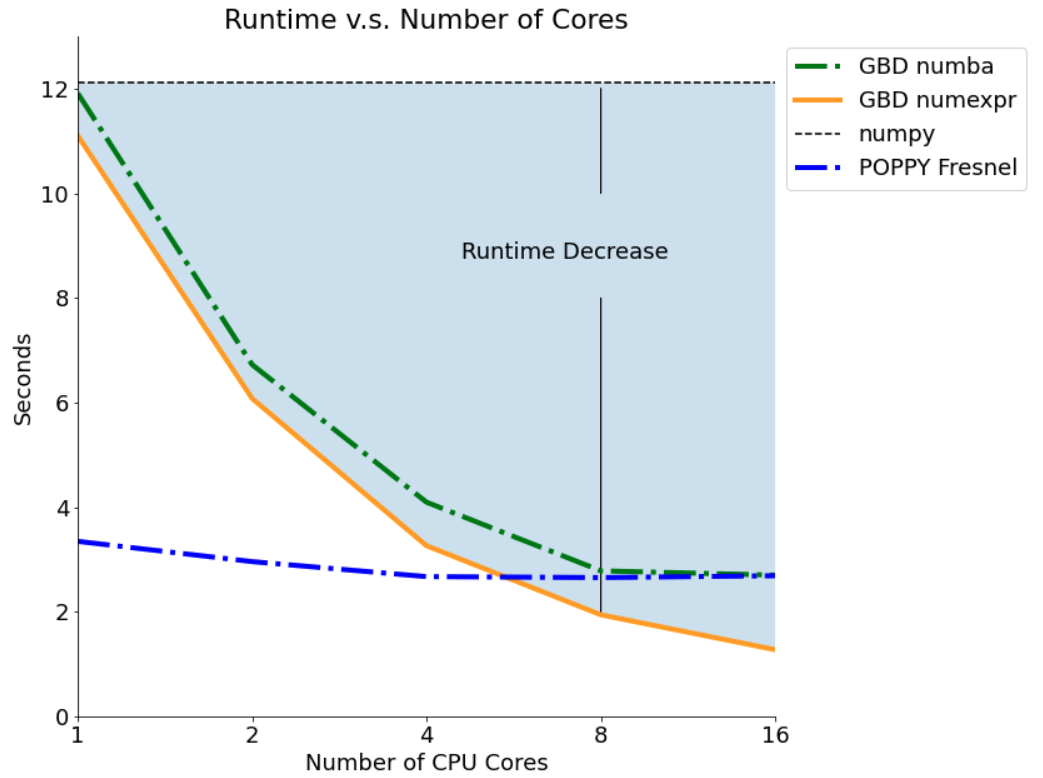
\includegraphics[width=0.7\textwidth]{gbdprofiling.png}
    \caption{Run time comparison for a 50x50 grid of Gaussian beamlets on a 256 x 256 detector grid v.s. number of CPU cores used. Numexpr considerably accelerates the exponential calculation given multiple processing cores, and is an encouraging path forward for further parallelization.}
    \label{fig:runtime_sim}
\end{figure}

\added{The vector operations used in the algorithm described in \hyperref[sec:algorithm]{Section \ref{sec:algorithm}} can be broadcasted across the entire array, enabling more efficient computation of the ABCD matrix. Broadcasting refers to the practice of writing code such that a given operation is applied to each element of the array simultaneously. This is more commonly known as "vectorized" computing. Our initial demonstration of the GBD algorithm was written using nested for loops (black, Figure \ref{fig:runtime_compare}), which was inefficient for highly-sampled simulations. Vectorizing our code resulted in a $\approx10\times$ decrease in runtime (blue, Figure \ref{fig:runtime_compare}). We then determined that the elementary matrix operations done using Numpy's linear algebra library were considerably dominating the runtime, so we wrote our own versions of the determinant, and inverse functions. This change resulted in a net $\approx40\times$ decrease from the original code written using nested loops (red, Figure \ref{fig:runtime_compare}). The runtimes for a simulation of various numbers of beams across the aperture to a 256$\times$256 pixel detector are shown in Figure \ref{fig:runtime_compare}.} 
\begin{figure}[H]
    \centering
    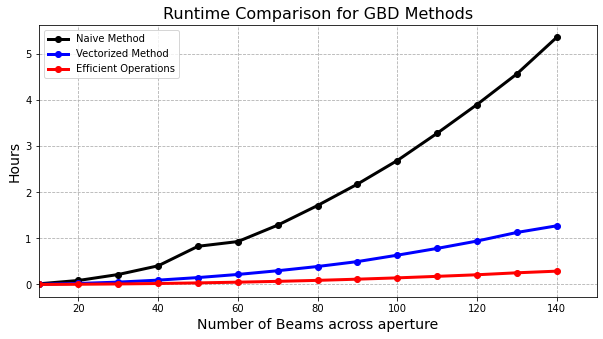
\includegraphics[width=0.7\textwidth]{runtime_vs_beamlets.png}
    \caption{\added{Runtime comparison of the iterations of the GBD algorithm applied in Python 3.8. The version using nested for loops is plotted in black, and high-beamlet simulations were computationally prohibitive. The runtime for the vectorized code is shown in blue, and the vectorized code with more efficient linear algebra operations (determinant, inverse) is shown in red. Overall, the decrease in runtime from the black curve to the red curve is $\approx 40\times$, which enabled the highly-sampled simulations in Figure \ref{fig:nonparaxial_coronagraph}.}}
    \label{fig:runtime_compare}
\end{figure}

We anticipate even greater speedups on GPUs. In particular, the creation of the phase array from the ray data is the slowest operation and needs to be parallelized for accelerated diffraction modeling. \added{Using the Cupy python package, adding support for GPUs was made quite simple given its compatibility with the numpy API. Preliminary experiments using our beamlet decomposition algorithm show a $\approx$16$\times$ decrease in computation time versus the algorithm shown in red on Figure \ref{fig:runtime_compare}. We have added GPU support though Cupy in our Poke package and plan to publish a formal study quantifying the degree to which GBD can benefit from accelerated computing in a future report.}

\section{\added{Code, Data, and Materials Availability Statement}}

The code used to conduct these simulations is located on the Poke repository on GitHub in the \verb"GBD_Paper" directory. The \verb"test_worku_transversal.py" script was used to conduct the simulations in this manuscript. These simulations were done during a very early release (v0.1.0) of Poke without much optimization for runtime or a user-friendly design. This version has been moved to the legacy branch of the repository as Poke and the GBD module is actively developed. \added{Presently, the updated version of this algorithm exists in Poke v1.1.0 as the poke.gbd module.}


